\documentclass[letterpaper,12pt]{article}
\usepackage[utf8]{inputenc}
\usepackage[spanish]{babel}
\usepackage[T1]{fontenc}
\usepackage{geometry}
\usepackage{graphicx}
\usepackage{enumitem}
\usepackage{color}
\usepackage{tabularx} % Aunque no se usa explícitamente 
\usepackage{float}
\usepackage{caption}
\graphicspath{{img/}}

% Configuración de márgenes
\geometry{
    left=2.5cm,
    right=2.5cm,
    top=2.5cm,
    bottom=2.5cm
}

\begin{document}

%%%%%% ENCABEZADO %%%%%%%

\noindent \textbf{Universidad Central de Venezuela}\\
\textbf{Facultad de Ciencias}\\
\textbf{Escuela de Computación}\\
\textbf{Organización y Estructura del Computador II}\\
Semestre 01-2026

\vspace{0.3cm}
\begin{center}
{\textbf{Práctica 2: Lógica Secuencial}}
\end{center}
\vspace{0.5cm}

%%%%%% CONTENIDO %%%%%%%

\begin{enumerate}
    
    %%%%% PREGUNTA 1 %%%%%
    \item Para cada una de las ondas de las figuras a continuación, dibuje la salida $Q$ de un \textbf{SR Latch}.
    \begin{enumerate}[label=\Alph*.]
        \item Caso 1:
        \begin{figure}[H]
            \centering
            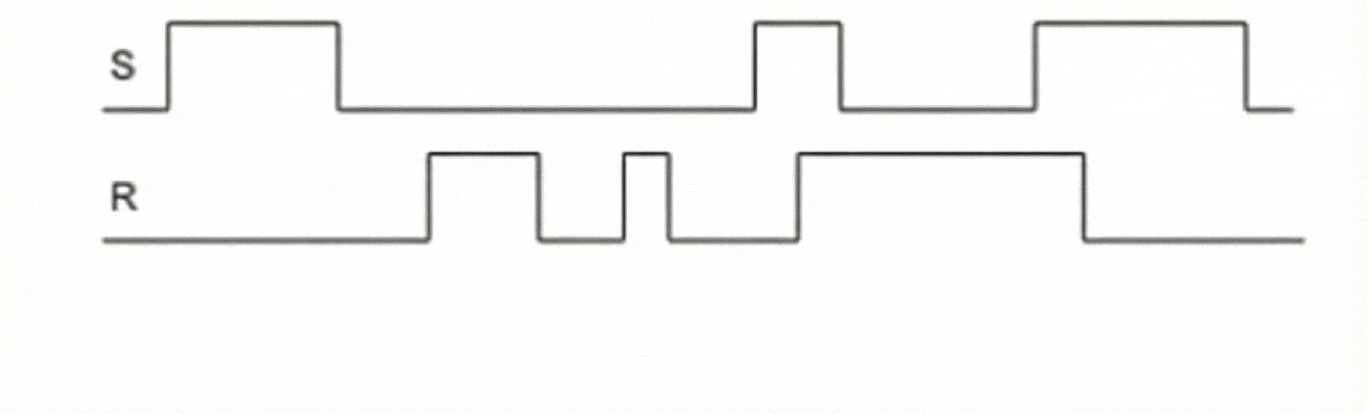
\includegraphics[width=0.8\textwidth]{FLIP-FLOPS/CASO_1.png}
        \end{figure}
        \item Caso 2:
        \begin{figure}[H]
            \centering
            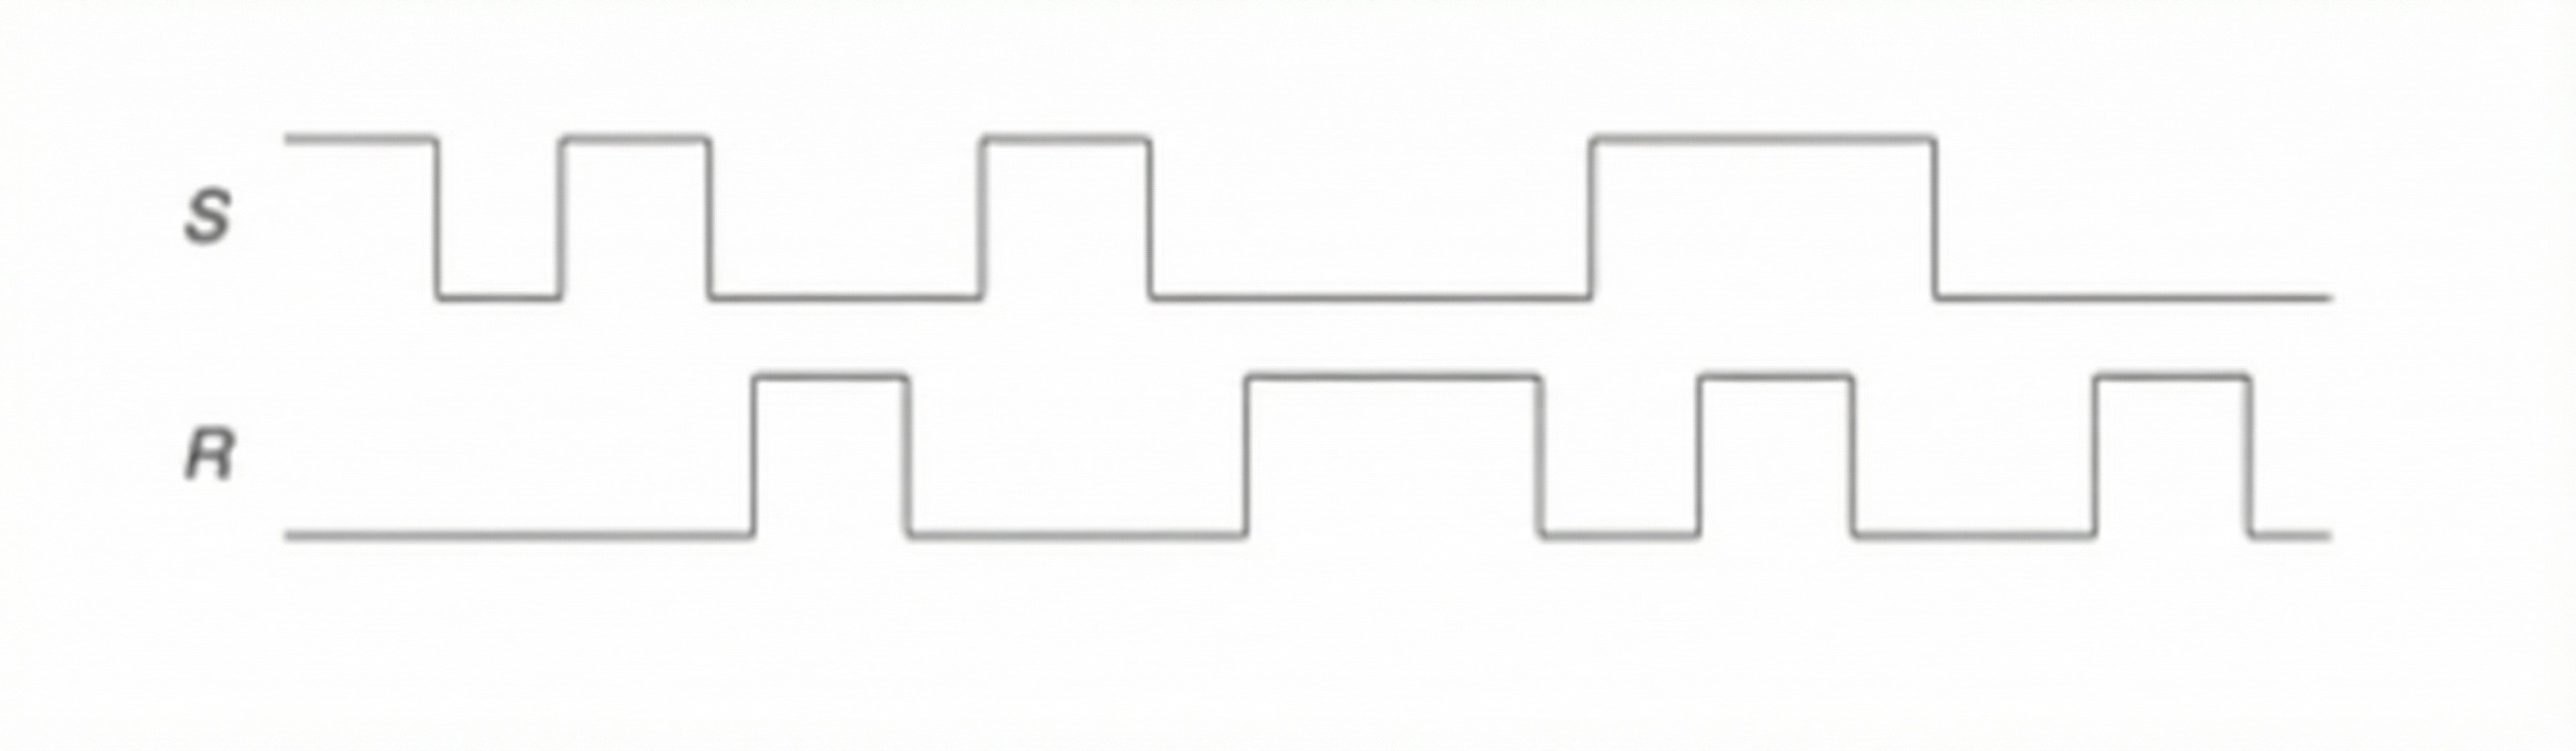
\includegraphics[width=0.8\textwidth]{FLIP-FLOPS/CASO_2.png}
        \end{figure}
    \end{enumerate}

    \pagebreak
    
    %%%%% PREGUNTA 2 %%%%%
    \item Para cada una de las ondas en las figuras a continuación, dibuje la salida $Q$ de un \textbf{D Latch}.
    
    \begin{enumerate}[label=\Alph*.]
        \item Caso 1:
        % Espacio para la figura B.1
        \begin{figure}[H]
            \centering
            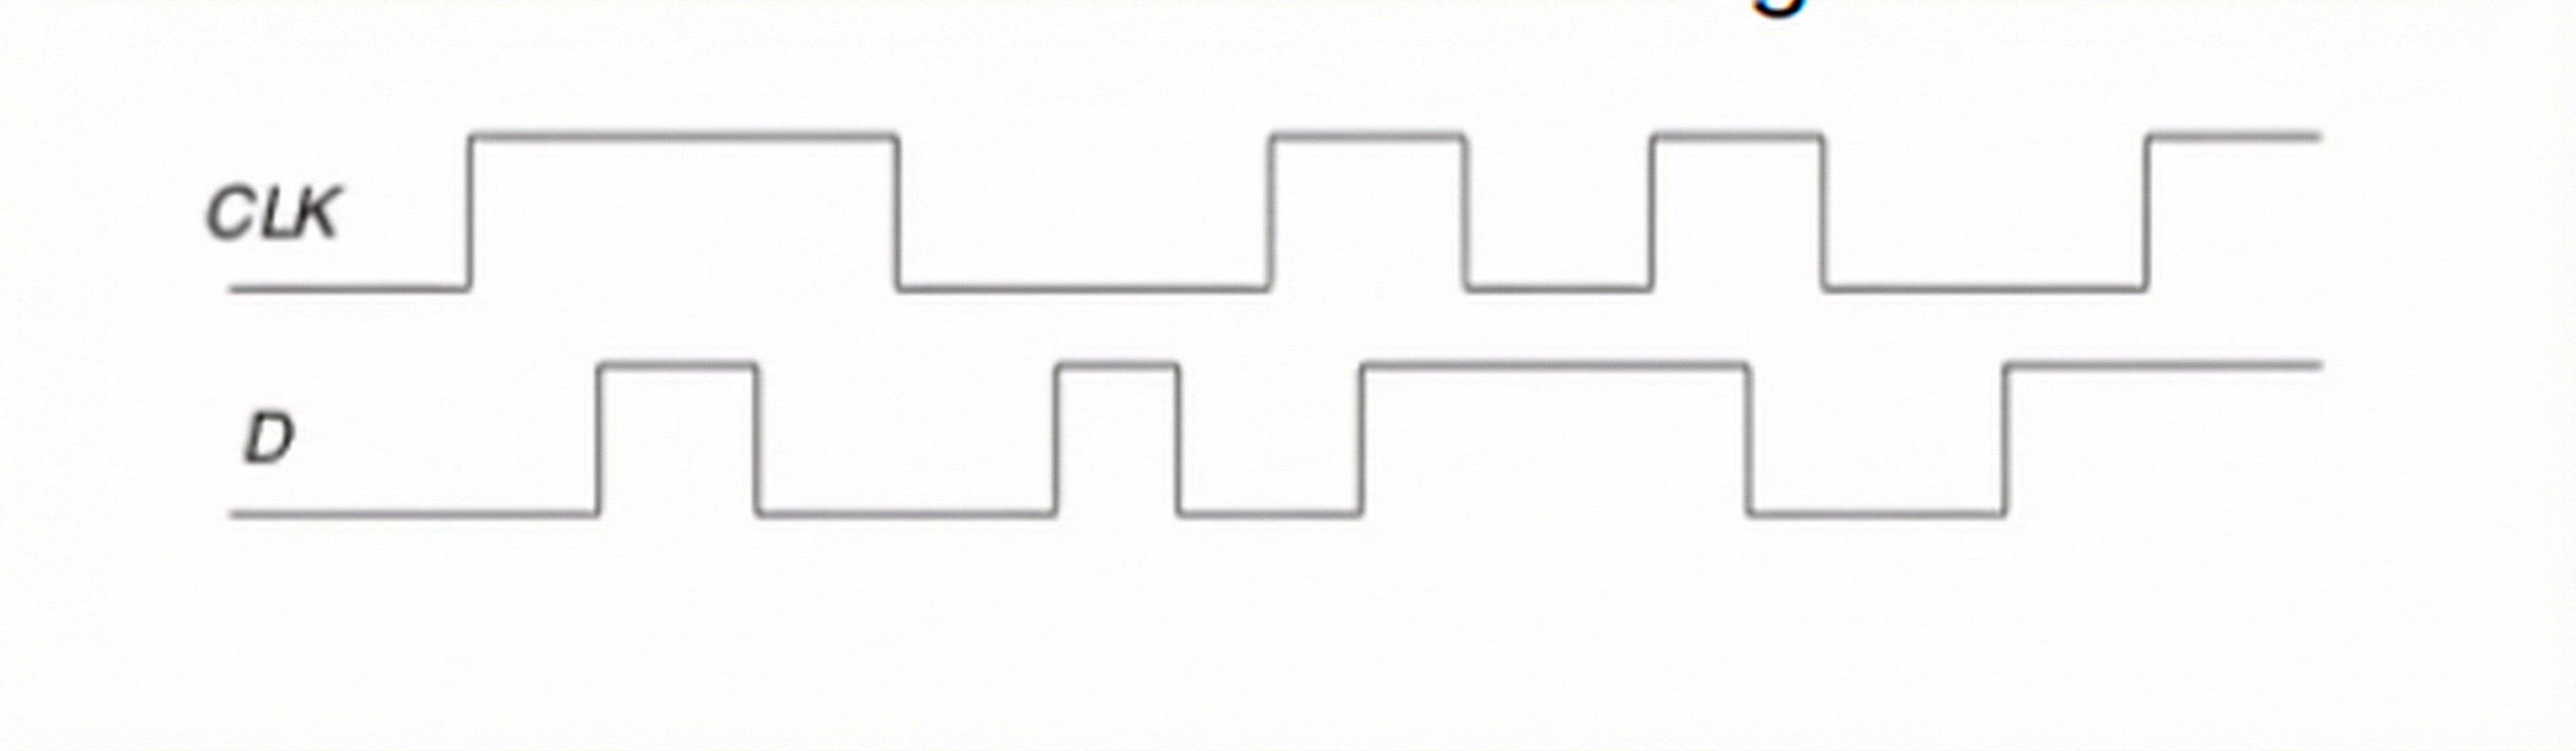
\includegraphics[width=0.8\textwidth]{FLIP-FLOPS/CASO_1_D.png}
        \end{figure}

        \item Caso 2:
        % Espacio para la figura B.2
        \begin{figure}[H]
            \centering
            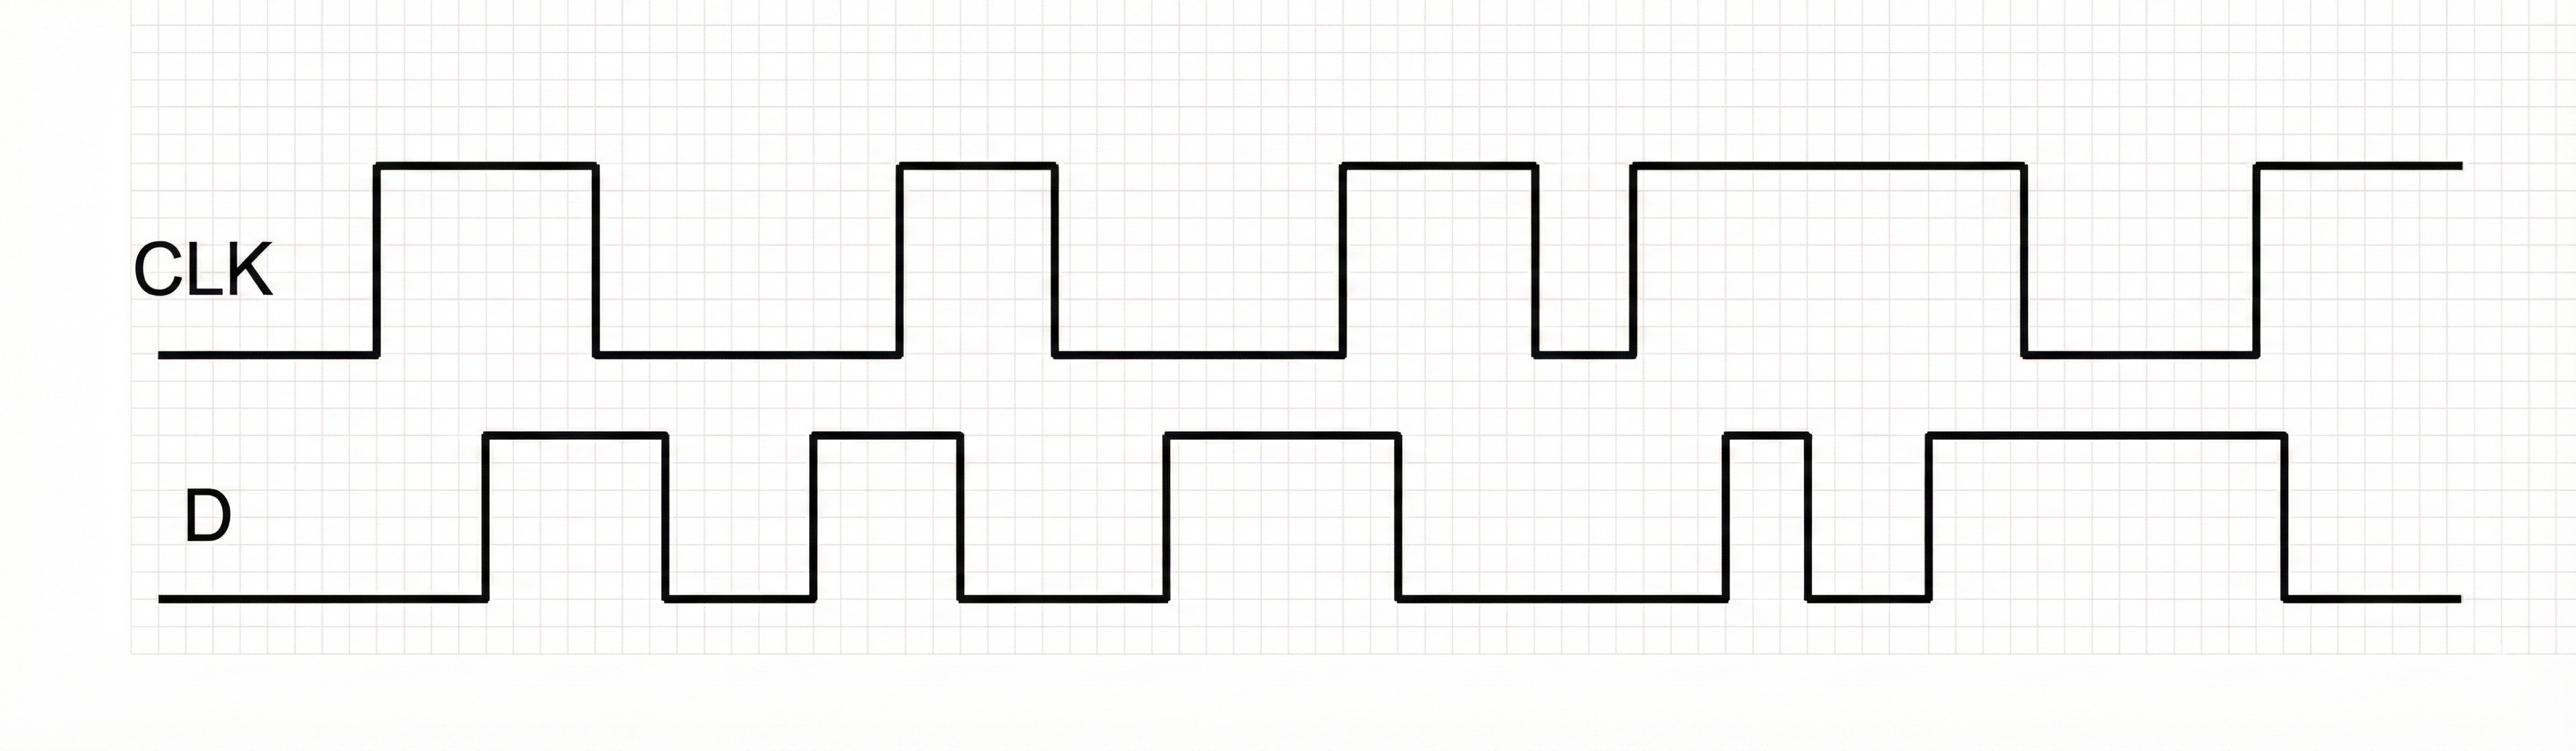
\includegraphics[width=0.8\textwidth]{FLIP-FLOPS/CASO_2_D.png}
        \end{figure}
    \end{enumerate}

    %%%%% PREGUNTA 3 %%%%%
    \item Dibuje la salida $Q$ de un \textbf{flip-flop D} empleando las figuras B-1 y B-2 anteriores.

    %%%%% PREGUNTA 4 %%%%%
    \item Un \textbf{flip-flop JK} recibe un reloj y dos entradas, $J$ y $K$. En el flanco ascendente del reloj, actualiza la salida $Q$. 
    \begin{itemize}
        \item Si tanto $J$ como $K$ son 0, $Q$ conserva su valor anterior.
        \item Si solo $J$ es 1, $Q$ se convierte en 1.
        \item Si solo $K$ es 1, $Q$ se convierte en 0.
        \item Si tanto $J$ como $K$ son 1, $Q$ se convierte en el opuesto de su estado actual.
    \end{itemize}
    
    Dado lo anterior se requiere que:
    \begin{enumerate}[label=\Alph*.]
        \item Construya un flip-flop JK usando un flip-flop D y lógica combinacional.
        \item Construya un flip-flop D usando un flip-flop JK y algo de lógica combinacional.
    \end{enumerate}

    %%%%% PREGUNTA 5 %%%%%
    \item Diseñe un \textbf{flip-flop D reseteable asíncrono} usando puertas lógicas.
    \vspace{3cm} % Espacio para dibujar circuito

    \pagebreak

    %%%%% PREGUNTA 6 %%%%%
    \item Para el diagrama de estados de la figura 1, realice lo siguiente:
    \begin{enumerate}[label=\Alph*.]
        \item Describa con palabras lo que hace la máquina de estados.
        \item Usando codificaciones de estado binario, complete una tabla de transición de es-
        tado y una tabla de salida para el FSM.
        \item Escriba ecuaciones booleanas para el siguiente estado y salida y dibuje un esquema
        de la FSM.
    \end{enumerate}
    \begin{figure}[h]
        \centering
        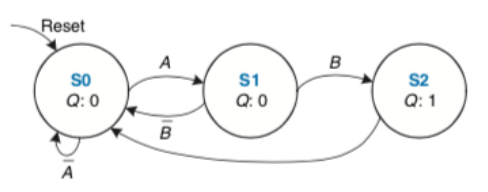
\includegraphics[width=0.5\linewidth]{FSM/EJERCICIO_1.png}
        \caption{Máquina de estado finito}
        \label{fig:placeholder}
    \end{figure}

    %%%%% PREGUNTA 7 %%%%%
    \item Para el diagrama de estados de la figura 2, realice lo siguiente:
    \begin{enumerate}[label=\Alph*.]
        \item Describa con palabras lo que hace la máquina de estados.
        \item Usando codificaciones de estado binario, complete una tabla de transición de es-
        tado y una tabla de salida para el FSM.
        \item Escriba ecuaciones booleanas para el siguiente estado y salida y dibuje un esquema
        de la FSM.
    \end{enumerate}
    \begin{figure}[h]
        \centering
        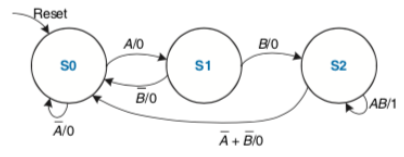
\includegraphics[width=0.5\linewidth]{FSM/EJERCICIO_2.png}
        \caption{Máquina de estado finitio}
        \label{fig:placeholder}
    \end{figure}

    \pagebreak
    
    %%%%% PREGUNTA 8 %%%%%
    \item Estas diseñando una FSM para realizar un seguimiento del estado de ánimo de cuatro estudiantes que trabajan en el laboratorio de OECII. El estado de ánimo de cada estudiante puede ser \textbf{FELIZ} (el circuito funciona), \textbf{TRISTE} (el circuito no funciona), \textbf{OCUPADO} (trabajando en el circuito), \textbf{ENREDADO} (confundido sobre cómo hacer el circuito) o \textbf{DORMIDO} (boca abajo sobre el teclado). Responda:
    \begin{enumerate}[label=\Alph*.]
        \item ¿Cuántos estados tiene la FSM?
        \item ¿Cuál es el número mínimo de bits necesarios para representar estos estados?
        \item ¿Cómo factorizaría la FSM para obtener múltiples máquinas más simples?
        \item ¿Cuántos estados tendría cada máquina más simple?
        \item ¿Cuál es el número total mínimo de bits necesarios en este diseño factorizado?
    \end{enumerate}

    %%%%% PREGUNTA 9 %%%%%
    \item Fuiste contratado para diseñar un dispensador de refrescos para la facultad. Los refrescos están parcialmente subsidiados por la escuela, así que solo cuestan 250 bolívares. La máquina acepta billetes de 50, 100 y 250 bolívares. Cuando se han insertado suficientes billetes, se dispensa la soda y el cambio si es necesario. Diseña una máquina de estado finito que pueda cumplir con esta tarea, las entradas de la MEF son 50, 100 y 250, indicando que billete fue ingresado, asume que se ingresa exactamente 1 billete en cada ciclo. Las salidas son “Dispensado”, “Regresar 50”, “Regresar 100” y “Regresar 200”. Cuando la máquina llegue a los 250 bolívares, debe dispensar el refresco y las salidas necesarias requeridas para dar el cambio correspondiente. Luego debe estar lista para empezar a aceptar billetes para otro refresco.

    %%%%% PREGUNTA 10 %%%%%
    \item Los Gray codes tienen la útil propiedad de que dos números consecutivos solo difieren en un bit. La figura 3 muestra un Gray code de 3 bits representando los números del 0 al 7. Diseña una máquina de estado finito que sea un contador modulo 8 para un Gray code de 3 bits que no tenga entradas y que tenga 3 salidas, (Un contador modulo N cuenta de 0 a N - 1 y luego repite, por ejemplo, un reloj es un contador modulo 60 para los minutos y segundos, ya que cuenta de 0 a 59.) cuando se resetee, la salida debería ser 000. En cada flanco de reloj, la salida debe ir al siguiente Gray code. Después de llegar a 100, debe ir a 000.
    
\end{enumerate}
\end{document}